\documentclass[a4paper,12pt]{article}
\usepackage[utf8]{inputenc}
\usepackage{amsmath}
\usepackage{graphicx}
\usepackage{hyperref}
\usepackage{float}

\title{RSS Feed Generator für Podcasts}
\author{Alwin Zimmermann}
\date{\today}

\begin{document}

\maketitle

\section{Ziel}
Das Ziel des Generators ist es, dass ein sogenannter Podcatcher den RSS Feed unseres Podcasts einlesen kann. Der RSS Feed muss hierfür von unserem Server als .XML (oder .rss) bereitgestellt werden. Bei einem RSS Feed gibt es einige wichtige Punkte zu beachten, die für den Aufbau eines syntaktisch richtigen Feeds beachtet werden müssen. Eine XML-Datei hat eine Baumstruktur, im Kopf stehen Infos wie: XML-Version, Encoding, RSS-Version.

\section{Struktur des RSS Feeds}
Nach dem Kopf steht die Channel-Sektion, in der der Channel die wichtigsten Werte erhält. Diese wären:
\begin{itemize}
    \item Titel
    \item Link zur Webseite
    \item Beschreibung
    \item Sprache
    \item Veröffentlichungsdatum
    \item Info, wann der Feed das letzte Mal erstellt/aktualisiert wurde
\end{itemize}
\newpage
Ab diesem Bereich beginnen die Items, in denen die Infos über die neuen Podcast-Folgen hinzugefügt werden können. Jedes Item (jede Folge) hat:
\begin{itemize}
    \item Titel
    \item Link zur Episode
    \item Beschreibung
    \item Enclosure URL
    \item Veröffentlichungsdatum
\end{itemize}
Nach allen Items wird der Channel geschlossen und der RSS Feed beendet.
\section{Probleme}
Das Paket \texttt{feedparser} (\url{https://github.com/kurtmckee/feedparser}) hat leider das Problem, dass es die sogenannte Enclosure URL nicht parsen kann. Diese ist jedoch essenziell für den Podcatcher, um die Datei finden zu können (Issue: \#285 enclosure not parsed). Das Problem besteht nicht beim ersten Erstellen des Feeds, sondern erst beim Wiedereinlesen des Feeds. Eine mögliche Lösung hätte sein können, die Infos alle redundant zu speichern, jedoch habe ich diese Lösung schnell verworfen, da sie mit einem unverhältnismäßigen Aufwand verbunden wäre. Eine weitere Lösung könnte das Modul RSS in Ruby sein, jedoch wollte ich die Problematik in Python lösen, da die meisten Teile unseres Projekts bereits in Python geschrieben waren und ich selber bisher noch kein Ruby geschrieben habe.
Deshalb habe ich mich für das Paket \texttt{lxml} entschieden, welches ein generisches XML-Bearbeitungstool ist (link: \url{https://github.com/lxml/lxml}). Dieses ist zwar nicht speziell für RSS entworfen, sollte jedoch manuell in der Lage sein, den Feed entsprechend anzupassen.
\newpage
\begin{figure}[H]
    \centering
    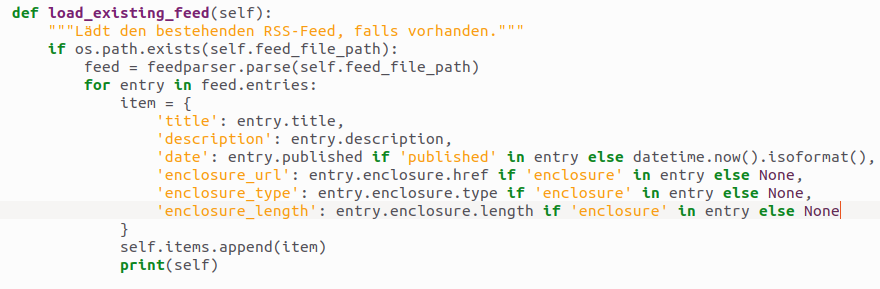
\includegraphics[width=1\linewidth]{Pics/BrokeFeedParser.png}
    \caption{Feedparser Bug}
    \label{fig:enter-label}
\end{figure}
\section{Das Script}
Das Script ist ein einfaches Python-Modul, das eine Funktion zum Hinzufügen von Podcasts in den Channel ermöglicht. Wichtig ist natürlich das Importieren der benötigten Python-Libraries.
\begin{figure}[H]
    \centering
    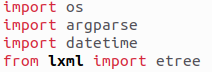
\includegraphics[width=0.25\linewidth]{Pics/RssImports.png}
    \caption{Imports}
    \label{fig:enter-label}
\end{figure}
Als Input-Werte benötigt es lediglich:
\begin{itemize}
    \item einen Titel als String
    \item eine URL zu der Folge, die hinzugefügt werden möchte
    \item eine Beschreibung der Folge
\end{itemize}
Das Veröffentlichungsdatum wird als aktuelles Datum gewählt, da das Script automatisiert ausgeführt werden soll. Zudem wird der Audio-Typ auf MP3 festgelegt, da wir das FLAC-Format von Anfang an verworfen haben. Mithilfe von \texttt{lxml} wird nun ein neues \texttt{<item>} Objekt hinzugefügt mit den angegebenen Werten.
\begin{figure}[H]
    \centering
    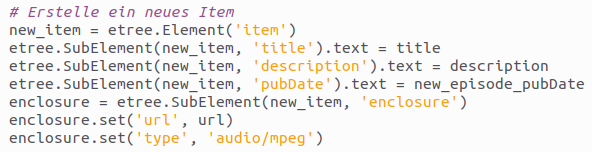
\includegraphics[width=0.75\linewidth]{Pics/RSSitem.png}
    \caption{New Item}
    \label{fig:enter-label}
\end{figure}
Auch wird im Kopf das \texttt{lastBuildDate} auf den aktuellen Moment abgeändert. Zuletzt wird der neue XML-Feed dann in einen Ordner mit dem Namen \texttt{rss} abgespeichert und kann vom Server publiziert werden.
\begin{figure}[H]
    \centering
    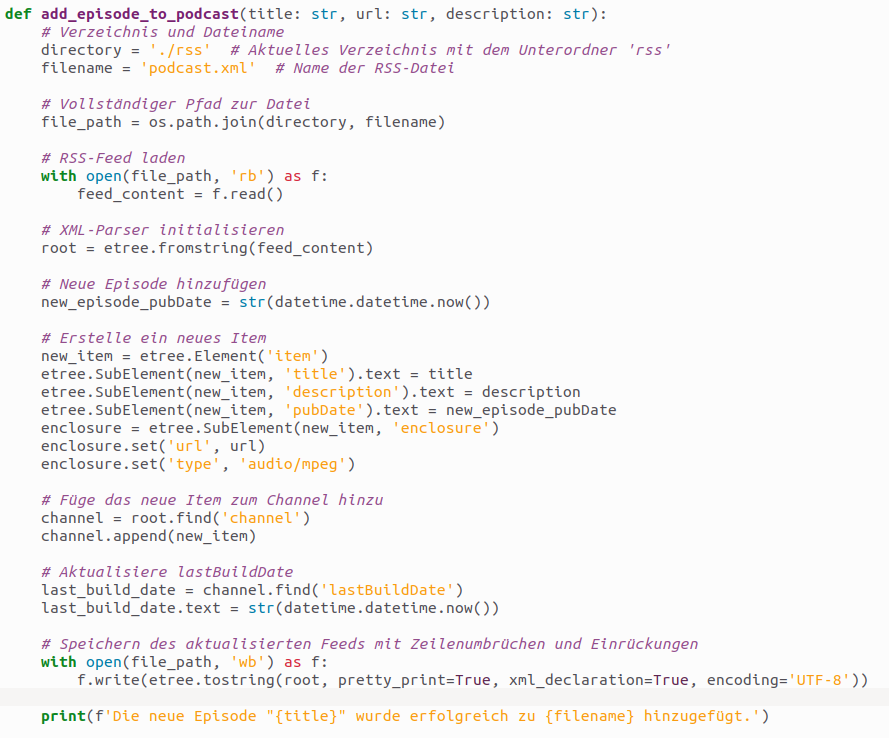
\includegraphics[width=0.9\linewidth]{Pics/RSSScript1.png}
    \caption{Script}
    \label{fig:enter-label}
\end{figure}
\footnote{Ich erkläre hiermit, dass ich bei der Erstellung dieses Projektes Unterstützung von ChatGPT, einem KI-gestützten Sprachmodell von OpenAI, in Anspruch genommen habe. Alle Inhalte wurden von mir überprüft und bearbeitet.}
\end{document}
